\documentclass[jou,apacite]{apa6}
\usepackage{textcomp}
\usepackage[utf8]{inputenc}
\usepackage[T1]{fontenc}
\usepackage{graphicx}
\usepackage{amsmath}
\usepackage{algorithm}
\usepackage[noend]{algpseudocode}
\usepackage{upgreek}
\graphicspath{ {./images/} }
\usepackage{listings}
\usepackage{color}
\definecolor{lightgray}{rgb}{.9,.9,.9}
\definecolor{darkgray}{rgb}{.4,.4,.4}
\definecolor{purple}{rgb}{0.65, 0.12, 0.82}


%JS definition
\lstdefinelanguage{JavaScript}{
  keywords={typeof, new, true, false, catch, function, return, null, catch, switch, const, let, if, in, while, do, else, case, break},
  keywordstyle=\color{blue}\bfseries,
  ndkeywords={class, export, boolean, throw, implements, import, this},
  ndkeywordstyle=\color{darkgray}\bfseries,
  identifierstyle=\color{black},
  sensitive=false,
  comment=[l]{//},
  morecomment=[s]{/*}{*/},
  commentstyle=\color{purple}\ttfamily,
  stringstyle=\color{red}\ttfamily,
  morestring=[b]',
  morestring=[b]"
}

\lstset{
   language=JavaScript,
   backgroundcolor=\color{lightgray},
   extendedchars=true,
   basicstyle=\footnotesize\ttfamily,
   showstringspaces=false,
   showspaces=false,
   numbers=left,
   numberstyle=\footnotesize,
   numbersep=9pt,
   tabsize=2,
   breaklines=true,
   showtabs=false,
   captionpos=b
}

\title{A Domain Specific IDE and JavaScript Comparison Engine}
\shorttitle{TIDE \& JeSSE}

\author{Gregory Mitten}
\affiliation{University of Sussex}

\abstract{
Although the modern IDE provides many useful features, it does not offer features designed to ease development in a specific domain. Some  would benefit greatly from an domain-specific IDE, often projects require much configuration and many developers solve the same problems repeatedly.  It is trivial for a domain-specific IDE to eliminate the former, simply provide a pre-configured environment. But to eliminate the latter these would first need to be identified,  if a system could identify these similarities, it could show code from similar code excerpts allowing developers to overcome their programming issues more expediently. This project hopes to develop a domain-specific IDE with such code comparison capabilities.}

\rightheader{Advanced Computer Science - Department of Informatics}
\leftheader{Gregory Mitten - University of Sussex}

\begin{document}
\maketitle    
                        
\section{Introduction}
\subsection{Problem}
\subsubsection{Context}
Tomorrow is a Copenhagen based start-up attempting to reduce the effects of climate change with their new mobile application, a prerequisite for the application to see widespread use is contributions from members of the open-source community. These volunteer engineers develop  JavaScript modules that provides the same functions interacting with various datasources, said modules are referred to as "integrations". Integration development offers a perfect environment to demonstrate the usefulness of a domain-specific IDE and code comparison engine, as the engineers share a code base and the same software problems. 

The company Tomorrow\textquotesingle s application, also named \textit{Tomorrow}, is soon to enter its beta. The React Native application aims to quantify the carbon impact of everyday actions, allowing users to comprehensively track their impact on the environment. How can \textit{Tomorrow} hope to handle all these vastly heterogeneous interaction modalities the user has with the climate? For example every day people: travel, eat, purchase various items, et cetera. How can one possibly personally quanitifed the transitive impact of purchasing a tshirt on the environment? \textit{Tomorrow} is relying on open source community to build what are known as "integrations".

An integration is a suite of functions written in JavaScript that connect to and retrieve data from a service, then parses it to match a schema. This integration can then be used by \textit{Tomorrow} to display the impact of said action(s) both graphically and textually 	mapping values to their carbon models. It should be evident that the development of integrations are a requisite step for the application to see wide use, hence it is pivotal an integration should be trivial to develop as not to deter any potential volunteer engineers.

\subsubsection{Definition}
Currently, in order for volunteer engineers to test their integrations, they must run a server locally which provides limited feedback and capabilities. This project’s aim is to reduce the initial discomfort, confusion and workload often present when beginning development on a system. The desired effect of this is to increase both the number of volunteer engineers and the volunteer engineer retention rate.

\subsection{Proposed Solution}
This project focuses on a technical route of achieving this outcome, attempting to automate the "toil" of integration development. Beyers et al \cite{beyerjonespetoffmurphy} refer to toil as work that is automatable Transpiling, hot loading, executing, rendering results, handling environment variables et cetera, these ideas will be explained later in greater detail. The notion is to eliminate the rigmarole often involved in project configuration, providing a pre-configured IDE with live servers ready to execute volunteer engineer code. 

Additionally, there are a few discrete ways to develop the interface functions (connect, collect and disconnect). As a consequent many there is likely to be a great deal of similarity between integrations. Necessarily the more integrations developed the greater the chance two of which are similar, and with Tomorrow anticipating over 100 integrations in an optimistic scenario it would be expected that a number of them to be very similar in places. Because of this, a code similarity engine is planned to allow Tomorrow and volunteer engineers to identify and learn from similar integrations. The volunteer engineers could use this to learn and fix their integrations, whereas the Tomorrow engineers may be able to, over time, refine their interface functions or add templates to further trivialise integration development.

\subsection{Relevance}
Although there is a much literature on code plagiarism detection and the modern IDE often provides information about when the code is duplicated. There seems to be a lack of focus on identifying similar but not equivalent code. It is often joked about that the contemporary software developer should concern themselves more with the literacy of sites like StackOverflow than they should with code. The reason this statement holds so much truth is software developers infrequently solve a unique problem. Although specific domain details make one problem superficially different, these are often easily identified by developers. It is hoped that this similarity identifying technology touches on an area largely unexploited, identifying similar code. In the future, this could be the basis of a JavaScript template engine facilitating the expedition of feature development. Many large technology companies use such technology internally but as of yet, there is surprisingly little use of these techniques in other spheres.

In this scenario, instead of thousands of engineers, many different languages and many different problems, instead there are few engineers, a single language and a ubitquitous goal. These constraints of the \textit{Tomorrow} integration development microcosm provide significant problem relaxation, it is hoped enough so that a similarity identification tool will be sufficiently performant to prove useful.

\subsection{Objectives}
The project focuses on two discrete areas, one
 of which is developing an IDE Web Application that eliminates all toil for volunteer engineers and can be used throughout \textit{Tomorrow\textquotesingle s }   lifecycle, the \textit{Tomorrow} IDE (TIDE).

The other domain is developing a performant code similarity tool, The JavaScript Comparison Engine (JeSSE).
\clearpage

\section{Background}
\subsection{Web IDEs}
The idea of an online IDE is far from a new one, many companies already offer this service: codesandbox.io, codepen and JSFiddle to name a few. However, typically these environments are for prototyping and experimenting rather than developing complete projects. Much of the literature involving remote code execution has a heavy focus on how secure systems are, this is not so much a concern with TIDE as there no sensitive data accessible or even associated with the IDE itself. It should be noted that security concerns involving inside integration code are assessed by the Tomorrow team and not by this project. Despite their security focus, previous solutions will be analysed to derive a set of best practices and technology considerations.

Some preach the benefits of an online IDE \cite{Aho2011}, namely the developer need not worry about configuring or updating the environment. They continue to suggest the use of a development server in which the code can be stored and executed on. A solution that aims to provide a comprehensive IDE experience in the browser is CodeAnywhere \cite{codeanywhere}, the system functions by providing each user with their own containerised virtual machine with dedicated memory and storage. This VM can be fully customised and set up with many development stacks and offering over 120 languages. As impressive as this solution may be spinning up a virtual machine for each volunteer developer this appears to be excessive for TIDE's scenario. 

Harvard have implemented a web IDE for students attending programming modules \cite{Malan2013}, known as CS50. CS50 is a much less distant scenario than a fully-fledged IDE  replacement and has many features akin to the requirements of TIDE. However, it does aim to provide many languages rather than just JavaScript. CS50 is built with node.js as its event-driven architecture is well-suited to handle asynchronous demands. Many developers may be concerned that a web IDE would incur non-trivial latency issues, enough so to make it worth using an offline alternative. Malan addressed this concern with the use of WebSockets for continuous interaction between server and client.

Goldman et al \cite{Goldman2011} developed a collaborative web IDE, they opted to import their text-based portion of the IDE in its entirety rather than engineering their own, this is very much applicable to TIDE. Building a web input for code complete with autocomplete and syntax highlighting would take up a great deal of development time and hence one of the alternatives they offer may be used. 

\subsection{Code Similarity}
There is a wealth of literature in code similarity with much of it focussing on detecting plagiarism, although the intent behind detecting code similarities may be vastly different from TIDE pragmatically there is little difference in technique. Often plagiarism detection is concerned with being fooled or deceived, JeSSE does not share this concern as integrations are not assessed,  hence worries of deliberate obfuscation are misplaced. Furthermore, the comparison scope is large for many of these tools often spanning university-wide and/or including previous years, whereas JeSSE will be used in a much more confined space. Regardless code plagiarism literature is regarded as extremely relevant.

There are several of the potential false flags (an incorrect assertion of plagiarism/similarity) involving lexical and structural code similarity, the relevant items for each are enumerated below \cite{Duric2013}.

Lexical
\begin{itemize}
  \setlength\itemsep{-0.5em}
  \item Modification of source code formatting 
  \item Renaming of identifiers
  \item Addition, modification or deletion of modifiers
  \item Modification of constant values
\end{itemize}

Structural
\begin{itemize}
  \setlength\itemsep{-0.5em}
  \item Changing the order of statements within code blocks
  \item Reordering of code blocks
  \item Modification of control structures
  \item Method inlining and method refactoring
\end{itemize}

The research that identifies these false flags follow a token-based analysis. In order to compile source code, the source code string is first transformed into a list of tokens by a lexer. In this instance these tokens are searched for longest contiguous match, this match must also be greater than specified value to avoid duplication, this approach is referred to as efficient randomized pattern-matching \cite{Rabin1987}. This algorithm is used in combination with a technique known as the Winnowing Algorithm, this strips white space from the tokens and forms n-grams from their hashes, these are then checked for a certain amount of overlap, for each value the hash with the lowest overlap is selected as representative. This reduces the number of hash values facilitating for greater efficiency in substring detection. They combine the results of the Winnowing Algorithm with efficient randomized pattern-matching to retrieve a final similarity value.

Earlier research \cite{Lancaster2005} completes a review of many source code plagiarism tools, they delineate plagiarism tools into two categories. Structure metric systems where every submission is extracted down to a vector of representative numbers and attribute counting systems, where certain attributes (such as identical values) are counted. Attribute counting systems to have greater accuracy when the programs were very similar however they were unable to detect partial plagiarism and overall the performance metrics for structural metric systems were much greater. 

Although it appears that many plagiarism identifiers are based on Token comparison there is an alternate approach in newer literature which involves a strategy of AST comparison.  An Abstract Syntax Tree is generated from \textit{parsing} the list of tokens generated by the lexer into a tree structure that represents the source code. Some suggest that token-based comparison is unable to effectively detect if the order of tokens has been rearranged \cite{Feng2013}, this problem does not occur if AST based comparison is implemented correctly. Their work uses an algorithm called AST-CC to hash nodes and compare the hash of each node with each other node with the same number of child nodes. Another tool \cite{Zhao2015} also opts to use an AST-based approach, in order to compare these nodes, they first transform the AST into a group into a linear list and then into a group of subtrees based on the number of child nodes. Once this is complete they also use the AST-CC algorithm over it for comparison. Their AST-CC hash function includes only the type and children of each node omitting other comparison considerations but certainly a more efficient solution for scale.

It has been found so far that comparison techniques unanimously use hashing for the comparison of nodes, however, it is believed, that this hashing although providing greater for comparison efficiency, ultimately obfuscates the weighting of "difference types". Differences can be delineated into a number of different "types", Listings 1 \& 2 demonstrate a difference of adding a line that was not found in the original code, this could be classified as one difference type called, for instance "add".  Listings 3 \& 4 show another potential difference type, called, for instance, "edit".

\begin{lstlisting}[caption=Difference type add - A]
console.log("Hello world");
\end{lstlisting}

\begin{lstlisting}[caption=Difference type add - B]
console.log("Hello world");
doX();
\end{lstlisting}

\begin{lstlisting}[caption=Difference type edit - A]
console.log("Hello world");
\end{lstlisting}

\begin{lstlisting}[caption=Difference type edit - B]
console.log("Another phrase");
\end{lstlisting}

Should a difference type of "add" and "edit" provide the same similarity value? This consideration and many others can be accounted for by using seperate penalisation values for each difference type, rather than tuning a hashing algorithm in which these values are much more obfuscated. Tuning the algorithms weights to provide more accurate similarity appears to be a powerful tool that needs to be considered. It should also be noted all of these previous tools were developed as plagiarism tools, as mentioned encountering slightly different problems. 
\subsection{Similarity Evaluation}

In order to compare the effectiveness of plagiarism detection systems many researchers employ other well-established systems, Duri\'{c} \& Ga\v{s}evi\'{c} use Measure Of Software Similarity (MOSS) \cite{aiken1994}. Research from \cite{Engels2007} found MOSS to be the most effective plagiarism system when utilised neural networks to assess the performance of 12 different engines, MOSS also invented the aforementioned Winnowing algorithm \cite{Schleimer2003} which is employed in MOSS. However, in order for MOSS\textquotesingle s values to have any meaning, the project must first be analysed to determine if it\textquotesingle s inner workings apply to this scenario.

MOSS is white space insensitive, suppresses noise by ignoring trivially short n-grams and is position-independent. MOSS does not opt to remove identifiers but instead replaces all identifiers with the character \textquotedblleft{}V\textquotedblright{}, but MOSS is sensitive to comments. Additionally MOSS uses asymmetric comparison, i.e. \texttt{compare(a,b)} does not necessarily have to yield the same result as \texttt{compare(b,a)}. 

\subsubsection{The Issue of Similarity}
Code similarity is not objective, although it may be asserted that two pieces of identical code are very similar, how many changes can one make before this similarity is lost? Plagiarism scarcely addresses this issue and instead defers to alternate plagiarism systems to provide answers, however, if other plagiarism systems are somewhat unsuccessful using as  a baseline is counterproductive. A solution to this issue, in order to tune his code similarity engine he used a list of code excerpts with code duplication and then manually checked whether they were duplicates \cite{Krinke2002}. Although this is somewhat hazier in the example of similarity manual checking must be used in absense of a formal definition. This \textit{Issue of Similarity} is referred throughout evaluation.

\clearpage

\section{System Decisions}
\subsection{Frontend Technology}
Choosing the frontend technology was fairly unimportant, the primary consideration was maintainability for \textit{Tomorrow} engineers, its capacity to support WebSockets and a library that functions as a code editor. JavaScript is the most widely used frontend language but a number of JavaScript frameworks met these criteria. As \textit{Tomorrow} develop their application in ReactNative it logically followed to use ReactJS for maintainability purposes. 
\subsubsection{Editor}
Considering the number of online code playgrounds it is somewhat surprising how few are available to be integrated into another project, many of these systems do not provide any autonomy into another environment. However, Microsoft has open-sourced their editing engine for VSCode, Monaco Editor, this has been imported and integrated into the frontend. 
\subsection{Backend Technology}
One of the most important considerations for the backend was how it handles the execution of JavaScript code, all languages except JavaScript itself must execute JavaScript with an external tool such as Google’s V8 interpreter (used in their browser Google Chrome) alternatively code can be executed using a node in the command line. It was deemed sensible to skip the middle man especially as node's non-blocking architecture combines with WebSocket best practices fluidly. The WebSocket framework chosen was socket.io as this is used in tomorrow, for ease of maintainability.
\subsection{Comparison Specification}
Taking into consideration the false positives specified earlier the final specification of the code comparison is as follows. The comparison engine ignores the following aspects of code.

\subsubsection{Location Data}
It is regarded as unlikely that exactly the same operations take place in exactly the same place, this does not mean that these items are code should not be considered similar. Not every operation is dependent on its location in a body of code.

\begin{lstlisting}[caption=Location independent example - A]
function connect() {
	const username = getUsername();
	const password = getPassword();
	
	return {username, password};
}
\end{lstlisting}

\begin{lstlisting}[caption=Location independent example - B]
function connect() {
	const password = getPassword();
	const username = getUsername();
	
	return {password, username};
}
\end{lstlisting}
In Listing 1 \& 2 we see semantically equivalent function bodies, the system should equate these two items as equivalent. Although counter examples can be provided where the location of line of code entirely changes its purpose, false positives are seen to be more acceptable than false negatives due to the fact human descretion is part of the process of identifiying whether code would be useful.
Location independence in this circumstance includes lines positions relative to each other and row and column numbers. 
\subsubsection{Identifier names}
Changing an identifier name does not effect how the code executes and hence it is not useful to penalise code excerpts for differences in these items.
Although there may be some similarities in the naming of functions many identical variables and functions may be given entirely different names and should not be penalised in similarity score due to this.
\subsubsection{Comments}
 Comments have no effect on execution, developer preference on commenting is irrelevant to semantic equivalence. If comments were supported some form of natural language processing would need to be included to effectively identify similar comments, as natural language is vastly more ambigious than code and the same measure of similarity will be very ineffective. Consider the comments in Listing 3 \& 4, these concerns are similarly applied to Identifier names.
 
\begin{lstlisting}[caption=Comment semantics - A]
//Deletes user data after use
\end{lstlisting} 

\begin{lstlisting}[caption=Comment semantics- B]
//Once all processes are finished with customer information, it is removed.
\end{lstlisting} 
 
  \subsubsection{Literal values}
Fetching data from different APIS will always involve different access strings, see Listing 5 \& 6. Accessing APIs is at the core of many of integrations. In other circumstances volunteer engineers may receive their data in a different measurement and need to transform it will involve different numbers but are essentially the same and still useful to learn from. Even though JavaScript is a dynamically typed language literals preserve their type information, this is the only information that should be stored about a value.

\begin{lstlisting}[caption=API access string dissimilarity - A]
http.get("https://supermarket.com/customer/CUST273/groceries?from=1564162882029")
\end{lstlisting} 

\begin{lstlisting}[caption=API access string dissimilarity - B]
http.get("shop.org/data?user=username&when=today")
\end{lstlisting} 
\subsubsection{Logging}
Logging should have no effect on execution, once again encounters the natural language issue.
\newline

These items are to be ignored indiscriminate of circumstance as to never impact similarity calculation. 

JeSSE will not attempt to test if two excerpts are strictly semantically equivalent. In this context,  strict semantic equivalence means that code excerpt a and b perform the same operations in the same order. Instead, semantic similarity is used, JeSSE aims to determine if two code excerpts are similar in their contents rather than entirely identical, as this will very seldom be the case. One of the primary reasons for using this loose definition is interface functions necessarily interact with an external, potentially proprietary system to retrieve their data. It is naive to assume that because two API endpoints appear to be similar they perform similar operations. 
All instructions that can potentially be called inside a method must be included, this is to say the nodes are collected regardless of conditional control structures. The engine must additionally support function inlining, elaborated upon later.

\subsection{Approach}
AST-based comparison was judged to be more suitable for this criteria as Feng et al mentioned location independence is ineffective in token-based systems. A structural based approach is also employed, the literature suggests this is more effective than its attribute-counting based counterpart. As this metric is not used internally to generate a binary condition like many of these tools the metric generated should be understandable by a developer with no background in code similarity.

\clearpage

\section{JeSSE Implementation}
\subsection{Preprocessing}
The code is first parsed into an AST, many JavaScript parsers are available however as babel is a de facto standard for transpiling (transforming source code to source code) ES2015+ code into the "ubiquitously" executable deprecated version (ES2015). If the project aims to support all JavaScript the babel parser should be used, as babel is actively updated for new JavaScript features, somewhat future-proofing the system. Once parsed all root-level functions are extracted from the AST,  in a well-formed integration this will include the interface functions and any member functions they call. All function nodes are preprocessed individually.

\subsubsection{Tree Flattening}
Each function is then recursively “flattened” from a tree into a list of its nodes, this is for ease of with the transformation of each tree into a structure in which they can easily be compared. This list includes each node and all their children but once the children are extracted from a node and added to the list they are removed from the node itself. Tree flattening takes into account all control structures, inner function to any degree of nesting. 

Flattening method takes two parameters, the top level nodes in each function body, and a list of all other member functions this is discussed in function inlining. The nodes types:

\texttt{IfStatement}, \texttt{WhileStatement}, \texttt{ForStatement}, \texttt{DoWhileStatement}, \texttt{FunctionDeclaration}

are referred to as “deep nodes” as they typically have children.

Deep nodes almost unanimously require leaf node extraction. The algorithm traverses through each node in the tree if children are present the parent node is added to the list and then its children are processed. As JavaScript uses pass by reference to accomplish this the node’s children are deep cloned, once this cloning has taken place the child nodes are then dereferenced in the parent to be cleared by JavaScript’s automatic memory management. The parent node is then added to the list of flat nodes, the child nodes are recursively passed into the flatten algorithm and the result is concatenated with the list. 

Other statements, such as lambda expressions, may also be deep nodes but they have a different structure. These nodes must pass a gauntlet of cascading conditions as there is so much diversity in the node structure there is no one simple condition to determine whether children are present. For example, if a node has a consequent, there is no certainty that consequent has a body and even if a consequent's body is present it may be empty. When a node succeeds in passing these conditions their children are extracted in the same fashion as deep nodes, but simply referring to a different route to the body. 

In Listing 1 \& 2 exactly the same instructions are called in a semantically equivalent manner but they would yield vastly different similarity results if function inlining was to be ignored. 

\begin{lstlisting}[caption=Function returning call expression]
function connect() {
	return getConnection()
}

function getConnection() {
	return http.get("https://api.com/get-session/username").execute();
}
\end{lstlisting}

\begin{lstlisting}[caption=Function returning contents of previous call expression]
function connect() {
	return http.get("https://api.com/get-session/username").execute();
}
\end{lstlisting}

Once function inlining is performed the resulting code bears a much greater resemblance, seen in Listing 3. JeSSE does not execute the code and so even though line 3 is unreachable it is still processed.

\begin{lstlisting}[caption=Function returning contents of previous call expression (function inlining of nodes)]
function connect() {
	return getConnection()
	return http.get("https://api.com/get-session/username").execute();
}
\end{lstlisting}

Function inlining is limited to member functions as to not exponentially expand the number of nodes being evaluated. In the other case where every method is processed,  the nature of programming abstraction this would almost certainly lead to an enormous number of nodes. This is not considered representative of the integration code, but rather every single operation that takes place within it. 

Each expression is analysed and if it is both (1) a call expression (2) and its method signature is present in the list of functions passed into the flattening method. The method name is then as a key to access the map of all member functions, it will then extract and flatten recursively the body of the called function. The result is the concatenation of the current list of nodes with the expression followed by the contents of the member function called. A function’s body can only be added to the list once per interface function, in the same manner, that the contents of a for loop are once rather than the number of times the loop iterates. 

As the list is not a list of every node called, rather a unique list of each node that can be called, a function’s body can only be added to the list once per interface function. Consistent with the manner that the contents of a for loop is not added the number of times the loop iterates (if deterministic).

\subsubsection{Eliminate Irrelevant Nodes}
The next phase of preprocessing is to eliminate the nodes that have been determined as irrelevant for comparison, which here only includes logging nodes. JeSSE has several specific logging method signatures hardcoded, the flattened node list is scanned and for call expressions matching these signatures dereferencing any matches.

\subsubsection{Eliminate Irrelevant Node Details}
Finally although some similarity tools replace information they do not want accounted for with a consistent token and others opt to simply ignore these components in their comparisons. JeSSE instead eliminates this information from the nodes entirely by dereferencing it, meaning all data in the remaining structure is to be considered. This must occur last as previous phases rely on this information. 

This completes pre-processing, Figure 1 \& 2 are examples of pre-preprocessing and post-preprocessing respectively.

\begin{figure}[h]
\caption{Parsed AST}
\centering
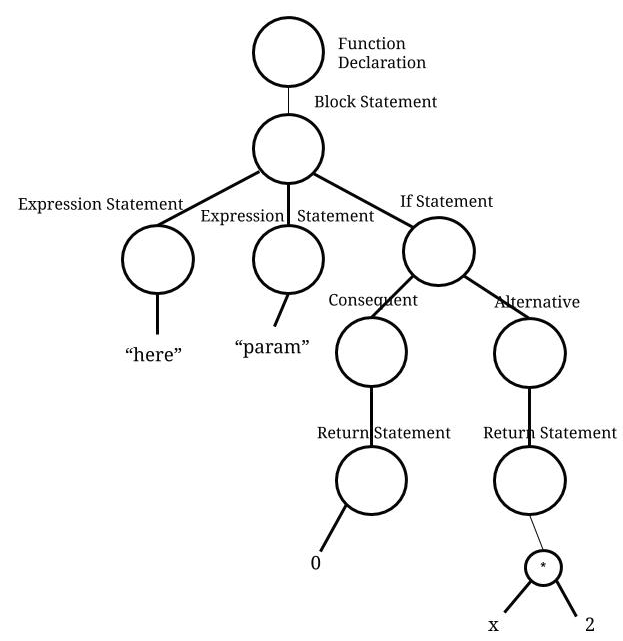
\includegraphics[width=0.5\textwidth]{ast1}
\end{figure}

\begin{figure}[h]
\caption{The AST after preprocessing}
\centering
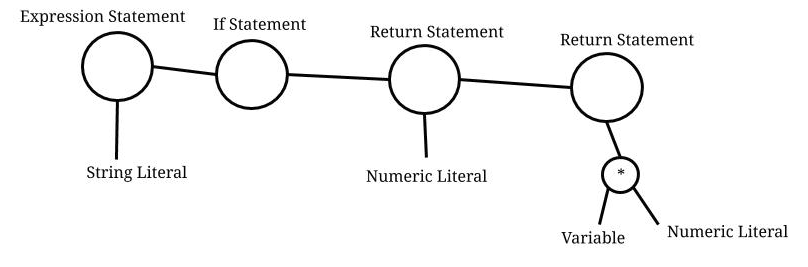
\includegraphics[width=0.50\textwidth]{ast2}
\end{figure}

\subsection{Comparing Function Bodies}
In order to compare function bodies, each node must find the node most similar to itself in the alternate list, node matches are exclusive, meaning each node can match with a maximum of one other node; this is true bilaterally. Once a list of these matches has been compiled the similarity of each can be calculated. The similarity value between any two nodes is calculated using a map of chosen values for each "difference type", the difference types chosen as well as an explanation of each can be found in Table 1.  The calibration of these values will be discussed later.
\newline\newline
Table 1
\begin{tabular}{l|p{50mm}}
  \hline
  Addition & A value is present in the compare
    node not found in the original node\\
  \hline
  Deletion & A value is not present in the compare node that is present in the original node\\
  \hline
  Edit & The field is present in both but different values are found\\
  \hline
  Array & An array is present in both places but a different number of values are found\\
  \hline
\end{tabular}
\newline\newline

Having control of how the system treats each individual difference in terms of the capacity to alter the punishment value is extremely valuable, although node hashing offers greater efficiency it is found lacking in this domain (without the creation of a specific hashing algorithm). On comparison of each node, fields are compared and the corresponding punishment values are applied, the punishment values of each node are summed. Note that although the comparison is similar to each base node can match with a maximum of 1 compare node, but if there are fewer nodes on one side than the other unilateral similarity calculator may say the functions are very similar despite the fact one is much smaller than the other. For example in Listing 14 would correctly identify the most similar node, found in line 1 of Listing 15, calculate only this similarity value and output that the items are identical. This is an unacceptable outcome and the systems must be appropriately penalised for missing lines, which is not yet accounted.

\begin{lstlisting}[caption=Shares one node only - A]
let start = new Date();
\end{lstlisting}

\begin{lstlisting}[caption=Shares one node only - B]
    let start = new Date().getTime();
    sleep(86400000);
    doX();
    doY();
    doZ();
    return new Date().getTime() - start;
\end{lstlisting}

Finding each node’s best match is far less trivial than it seems. If this is done naively the match of one node will erroneously prevent all future nodes from matching with that node regardless of whether their similarity is greater than the original match, this only occurs due to the exclusivity of the problem. One solution to this would be to compare these values and if the new node shows greater similarity then return and repeat the process with the initial node. This results in unnecessary processing. The preferred solution that has been chosen is an algorithm developed named "exclusive match".

Exclusive match builds a hierarchy of matches ordered by similarity as the nodes are compared. Each difference type is assigned its corresponding value and these are summed to form the similarity value, due to the nature of the parser two ASTs can contain vastly different keys despite not being extremely different in nature on occasion, so an upper boundary has been set as a maximum difference punishment value. Once all hierarchies have been built, the uniqueness of the first item in each hierarchy is then tested for duplicates. If a duplicate is identified a loop is entered, the loop will continually remove the highest ranked item from the hierarchy with the lower similarity value. This continues until the first index in the current node's hierarchy in the hierarchy it is either: Unique or has the highest similarity value of all it's duplicates. Figure 3 represents the first phase where all hierarchies are built, Figure 4 represents the hierarchies once duplicates are eliminated.


\begin{algorithm}
\caption{Exclusive Match}\label{euclid}
\begin{algorithmic}[1]
\State hierarchies $\gets \textit{[]}$
\For {each node $n$ in $nodes$}
	\State hierarchies.add(sort(match(node, compareNodes))
\EndFor

\For {each hierarchy $h$ in $hierarchies$}
	\While{$compareResult \neq  0$}
		\If{$compareResult = 1$}
		\State hierarchies[h].pop()
		\ElsIf{$compareResult = $-$1$}
		 \State hierarchies[compareResult.index].pop()
		\EndIf
		\State $compareResult \gets compare(h, hierarchies)$
	\EndWhile
\EndFor
\Procedure{match}{$node$, $compareNodes$}
\State hierarchy $\gets \textit{[]}$
\For {each node $cn$ in $compareNodes$}
	\State hierarchy.add(similarity(node, cn.AST), cn.idx)
	
\EndFor
\EndProcedure

\end{algorithmic}
\end{algorithm}

\begin{figure}[h]
\caption{The hierarchies built for each node}
\centering
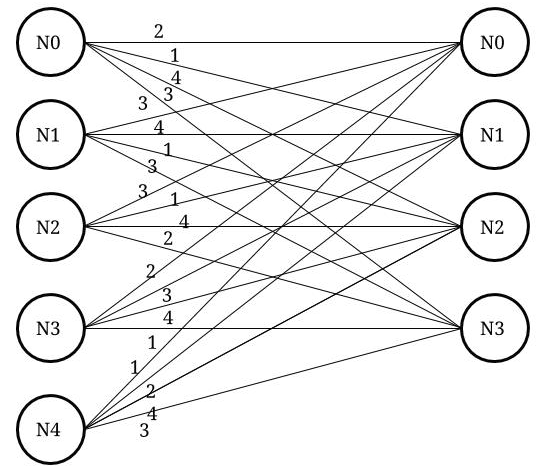
\includegraphics[width=0.50\textwidth]{allhierarchies}
\end{figure}



\begin{figure}[h]
\caption{The hierarchies with pruned duplicates}
\centering
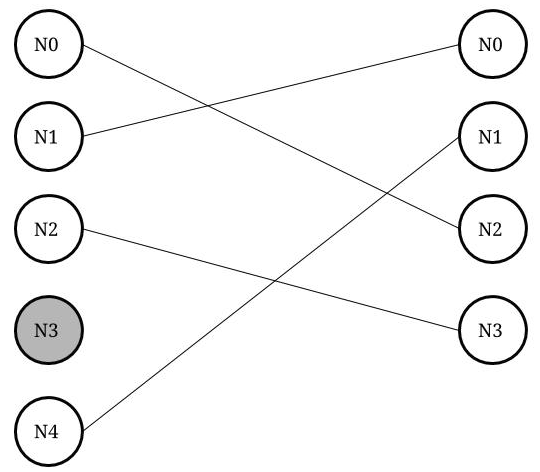
\includegraphics[width=0.50\textwidth]{hierarchies}
\end{figure}

Upon completion, populated hierarchies are summed and stored including their similarity values. Empty hierarchies are not simply ignored, these items are identified and their count is used as a modifier to multiple $S$ (The similarity value) by (where a lower $S$ represents greater similarity).  

To make $S$ relative to its size of the nodes that generated it the total $S$ of each function is divided by the number of keys present in all of its nodes. Key-count is always directly proportionate to the comparison as deep-diff works on the basis of comparing each individual key in the node. What this does mean however is that more complicated nodes are weighted heavier in the generation of $S$ but this was seen as appropriate.

Once a score is generated for a function in the form \texttt{compare(a, b)} only one side of the comparison has taken place and the system is unilateral. This result is weighted as 50\% and the other half is derived from an inverse comparison for \texttt{compare(b, a)}.


The purpose of this transformation is so the engineers perceive the value as a percentage, this should intuitive to the engineers without much thought. Although it should be noted that a $TS$ of 75 is not 75\% similar, it was judged this is representative enough that engineers will get the general idea of the system. JeSSE has been tweaked so an $S$ greater than 1 is seen to be very dissimilar and will be displayed to volunteer and \textit{Tomorrow} engineers alike as 0. If these values are displayed in such a way why even give multiple pieces of code the possibility of having a difference value less than 0? This is because as the most similar integration must still be selected i.e. a dissimilar function of similar length is still considered more similar than the contrary. Providing a $TS$ to the engineer of -56 was judged to be confusing and break the percentage-based illusion, after all how could the code be -56\% similar. $TS$ for each method is displayed alongside a visual indicator of similarity client-side and a copy of the most similar code to allow the developer to inspect it to look for places they could complete their task differently. 

Each method of each integration undergoes the comparison process with the volunteer engineer's code, matching each function to the corresponding interface function. After every function has been assessed the code is imported from the most similar integration for each interface function, to prevent memory leaks these modules must be deleted. First emitted to the client-side to reduce further waiting time and then the modules are removed from the cache.

\clearpage

\section{TIDE Implementation}
\subsection{Code Execution}
There are many ways to dynamically execute code in JavaScript, one of which is the notorious \texttt{eval()}, many of the reasons eval is widely disliked is due to its security implications, not particularly concerning to TIDE. However,  it also runs into many efficiency concerns. Meawad \cite{Meawad2012} asserted that \texttt{eval()} is, in almost every scenario, replaceable by a superior alternative, even developing a tool that automatically replaced 97\% of eval usage. There are many alternatives to \texttt{eval}, some are assessed below.

\begin{itemize}
  		\setlength\itemsep{-0.2em}
		\item JavaScript provides a text parameter for its Function class allowing the passing of source code directly into the object, i.e. \texttt{new Function(“console.log(‘test’)”).apply()} prints \texttt{test} in the console. This appears to be a thinly veiled eval it is not quite, the code input here is parsed into a JavaScript Function whereas eval runs the input expression with whatever scope it is called in. The issue with passing code in only functions can be passed in whereas the volunteer developers code entire modules with constants and imports which will not have the correct scope inside a wrapper function.
		\item Another strategy is by Document Object Model modification, this would involve appending the script to the HTML of the current page their viewing and then running the methods from the JavaScript initially provided, besides the fact this solution is inelegant and would likely be very error-prone there are additional reasons why this should not be used. The first of which is it would require their browser to support the JavaScript they are writing, although this may seem like a reasonable request it is not unlikely some experimental feature is used for some element of their integration that is not supported by many old versions of browsers. Finally, there are numerous modules which may be imported from the \textit{Tomorrow} project which would be programmatically awkward to selectively provide based on the DOM. 
		\item Although node.js is a JavaScript framework perhaps it is better practice to write the code to a file stored on the backend and then initiate JavaScript execution via the command line using a tool such as Google’s V8 JavaScript interpreter. However, retrieving the console output is regarded to be inconsistent and cannot possibly be the best solution.
		\item The final and perhaps only viable idea is to provide the code to the backend, write it to a file, treat the file as a normal module and import it. This must be synchronous of course due to the race condition of the file being populated. But once this is complete the code will be indistinguishable from a module imported on boot, allowing for the full capabilities of a module. Meaning the results do not need to be parsed or converted, they will natively retrieve JSON objects that can be directly sent to the client.
		
	\end{itemize}
	
			Once the module importing option was decided upon a new problem arose in order to allow execution of all valid JavaScript, the system must support also support ES2015+ syntax. However, node.js does not yet have full native support for all these features \cite{node.js2019}. One solution to this is transpiling the code, from ES2015+ to ES2015 as ES2015+ does not add any feature to the language which cannot be replicated in more verbose ES2015 \cite{Silva2017}, which is fully supported by node.js. However, transpiling comes at a cost, all code must be transformed before execution this is in most cases a trivial issue as all code is transpiled at the beginning. In this circumstance as ES6 features are supported in the IDE every single code execution must be transpiled to ES2015 to run, a non-trivial performance cost. Another and perhaps better solution to this is via the use of ESM, a module loader that transforms ECMAScript2015+ modules at run time rather than transpiling them \cite{powers2018}. This can be added to the entire system via simply running the server's root JavaScript file through the ESM module loader rather than directly. The elegance of this solution comes from the issue that the server itself uses ES16+ syntax,  the ESM module loader combats both this and the issue of ES16+ in integrations simultaneously.
			
				\begin{figure}[h]
\caption{The Code Execution flow}
\centering
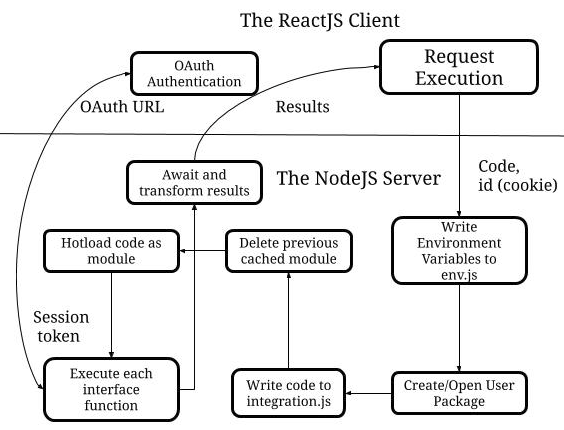
\includegraphics[width=0.55\textwidth]{codeexecution}
\end{figure}
			
			Figure 5 represents the phases each code execution passes through when an execution request is sent from the user. This was achieved using a promise chain, of course, some items on the list are conditional, i.e. a user package is only created if one currently does not exist. The environment is set up as an empty module exporting the fields specified by the user as a JSON Object. Additionally, in order for the stub to have its methods made accessible,  code specifying all interface functions as exports is appended.

All integrations imported with ES2015 dependency management system, rather than with ES16. However, the integrations themselves may import the modules using whichever syntax the volunteer engineer chooses, this is facilitated by the ESM module loader.  ES15+ \texttt{import} statement specifically makes the dependency cache inaccessible during run-time.  Even with ES2015's require, modules are cached and even if it is explicitly stated that the module should be reimported node will simply retrieve this cached version. In order to facilitate dynamic hot-loading multiple times in a session, the system must resolve the cached module and dereference it, it can then be re-imported. 

Once imported the module's interface functions are executed, feeding them arguments identical to what they receive in tomorrow. The \texttt{connect} interface method receives parameters in the form of two functions, the first of which is the app fetches the username and password of the current user. In the IDE the volunteer engineer must instead fill out an authentication panel. The other method requests a web view to be resolved for OAuth, discussed later. 

The outcome of the connect method is stored and then passed as the state parameter into collect, once this is complete the remainder of the operations benefit greatly from node.js's asynchronous nature. The calculation of code similarity, the transformation of the \texttt{collect} result in various representations and fetching the logs takes place simultaneously. These results are emitted to the client.
\subsection{Miscellaneous Features}
\subsubsection{Concurrency}
To allow many volunteer developers to access the system simultaneously, each user will be assigned a unique id as a cookie upon their first entry into the site, this id is used to generate their session package. A user package has all the necessary file components for one to develop: their simulated environment and the module, user packages are persistent as long as their corresponding cookie is, meaning that their code is stored on the server rather than locally on the browser. These ids must be generated in such a way that it is extremely unlikely one user should be able to guess the id of another user to interfere with their integration, because of this a Universally Unique Identifier (UUID) is used.

\subsubsection{Logging and Debugging}
For TIDE to see any long-form use, it must provide adequate information for debugging. This presents an issue and is clear why a virtual machine is used in the case of some web IDEs, the execution of the code is controlled by a server with a console that is not accessible. If volunteer developers are to have any idea why their code is not behaving as expected, they must have a means of receiving error messages or retrieving values in the program. Execution state, whether successful or otherwise is provided to the volunteer engineer using pop-ups, if no meaning error name can be found the message “an error occurred but not message could be retrieved appears” this was judged to be better than no message at all.

To implement logging a very simple class was made available to the user, they simply import a logger class from the project files (a path is specified in the IDE documentation) and then build a stack of logs by calling functions within the logger. Typical logging levels are provided such as ‘info’, ‘debug’, etc. To access these logs and return them to the client-side, a logger is then added to the export function of the aforementioned module stub. However, due to the fact, the logger's presence is not guaranteed an additional line must be appended to the module exports, the contents of "logger" whether present or not and exports that instead.

\subsubsection{Execution Results}
Once the user has executed their integration they must be able to view the results, several display formats will be returned to the user. The first of which is a graph mapping the co2 usage over time allowing them to visualise their data as a time-series. Next cumulative co2 emissions will be mapped using an appropriate carbon model (provided by Tomorrow) to see if their results are reasonable. Finally, their data will be returned in raw JSON, the response the programmer might expect to see initially. 

\subsubsection{OAuth}
Volunteer engineers are able to use OAuth in their integration, this is where the differences in the nature of server-based code execute become more evident. In order to initially resolve the web view to a value, i.e. a session token, the volunteer engineer must often enter values into this web view. This, of course, presents an issue as their code is tested on the node.js server making the volunteer engineer entirely unable to continue this process and leaving the system frozen. 

The OAuth flow was implemented with the use of WebSockets, the request is initially sent via HTTP to the backend which will then begin the execution cycle as normal. Once the connect interface method is called a well-formed OAuth integration authorisation takes place via a web view,  a promise is set up on the server that emits a signal to a receiving client-side WebSocket. On receiving this transmission the client creates a new window using the URL provided by the server, providing a means for the volunteer engineer to enter their authentication information. Once the user has logged in to the window (this can also take place automatically if details are stored) the server-side promise resolves as it receives a response from the client and can continue execution with valid authentication.

\subsubsection{State Injection}
Some volunteer developers may not want to run the \texttt{connect} component of their system on occasion, this may be to probe the system for a bug or perhaps because their API has a finite number of calls not well-suited to the development of the system. The \textit{Tomorrow} application itself will also rarely authenticate, instead opting to store this information where possible, hence engineers may be interested in testing the more likely circumstance of connection state already existing. 

In a client-side modal, volunteer engineers can specify well-formed JSON (enforced by component) that is passed as a parameter with the code into the server. If this state injection is present the server bypasses the execution of certain features and instead only executes the \texttt{collect} method, using the state provided. This may also be convenient for providing expired tokens for testing.

\subsection{Testing}
System testing is primarily focussed on the code similarity element of the project. This is a perfect domain for unit testing, the comparison engine produces an output of a float ($S$) indicating the two functions are considered identical. Many of the requirements of JeSSE are specified in such phrasing as “the inclusion of x should not affect the outcome of the comparison”, because of these tests could be created in such a manner. Some such tests include:

\begin{itemize}
  		\setlength\itemsep{-0.2em}
		\item Same nodes in a different order
		\item Same nodes in a different order with some inside control structure 
		\item If statement child nodes are flattened
		\item For loop child nodes are flattened
		\item ... for all deep nodes
		\item Lambda expression content flattened
		\item Logging nodes are ignored
		\item Comments are ignored
		\item Called functions are inlined
	\end{itemize}

\clearpage

\section{Hyperparameter Tuning}
The final phase of optimising JeSSE involves tuning various numeric hyperparameters. (1) The Missing modifier increment, for each missing match increase a modifier by this value, this modifier is ultimately multiplied with the similarity score. This is used as it was judged to be logically more effective in identifying similarity, for every missing line the code becomes less and less likely to be largely similar. (2) Difference values, the similarity punishment value assigned to a specific difference type. (3) The maximum punishment value one node can receive, some nodes can be so expansive punishment values are disproportionate see Listing 4 \& 5.

\begin{lstlisting}[caption=Function returning contents of previous call expression]
function sleepTest() {
    let start = new Date().getTime();
    sleep(1000 * 60 * 60 * 24);
    return new Date().getTime() - start;
}
\end{lstlisting}

\begin{lstlisting}[caption=Function returning contents of previous call expression]
function sleepTest() {
    let start = new Date().getTime();
    sleep(86400000);
    return new Date().getTime() - start;
}

\end{lstlisting}

If no maximum punishment value is set here, due to the manner that JeSSE recursively evaluates nodes even inside of call expressions this produces an $TS$ of 30, which has been regarded as disproportionately low for such a change. A naive solution to this is to say why not treat all numeric operations and such as one numeric literal, the calculation in listing 4 is trivial and present for clarity sake but in real integrations, it is unlikely all calculations will be deterministic.

\subsubsection{Combinatorial Tuning}
Although there is little doubt an approach of assessing combinatorial parameters thoroughly  would lead to the system functioning more effectively, due to the oracle problem brought about as a result of the problem of similarity an enormous amount of manual work. This will be discussed further later on.

\subsection{Test Suite 1}
A test consists of comparison between $n$a and $n$b
\begin{lstlisting}[caption=Comparison 1a \& 1b - Identical]
	let x = true;
\end{lstlisting}

\begin{lstlisting}[caption=Comparison 2a - Let against const]
	let x = true;
\end{lstlisting}
\begin{lstlisting}[caption=Comparison 2b - Let against const]
	const x = true;
\end{lstlisting}

\begin{lstlisting}[caption=Comparison 3a \& 3b - Identical extended]
	let x = true;
	if (x) {
		functionCall("here");
	}
\end{lstlisting}

\begin{lstlisting}[caption=Comparison 4a - Effect of numeric literal vs numberic expression]
	let x = true;
	if (x) {
		return 50;
	}
	return 0;
\end{lstlisting}

\begin{lstlisting}[caption=Comparison 4b - Effect of numeric literal vs numberic expression]
	let x = true;
	if (x) {
		return 25 * 2;
	}
	return 0;
\end{lstlisting}

\begin{lstlisting}[caption=Comparison 5a - Similar functions with literal and identifier name changes]
	let url = "https://api1.com/apiKey=" + state.API_KEY + "&data=search-data";
	return http.get(url);
\end{lstlisting}

\begin{lstlisting}[caption=Comparison 5b - Similar functions with literal and identifier name changes]
	let BASE_URL = "api2.co.uk/key=" + env.API_KEY + "&search=data";
	return superagent.get(url);
\end{lstlisting}

\begin{lstlisting}[caption=Comparison 6a - Real integration connect bodies]
    const { username, password } = await requestLogin();
    const { customerId } = await getUser(username, password);
    const associatedMeteringPoints = await getMeteringPointAssociated(
        username,
        password,
        customerId
    );
    if (!associatedMeteringPoints.length) {
        throw new Error("No associated metering point found");
    }
    const meteringPointId = associatedMeteringPoints[0].mpid;
    const priceRegion = await getRegion(meteringPointId);
    // Set state to be persisted
    return {
        username,
        password,
        meteringPointId,
        priceRegion
    };
\end{lstlisting}

\begin{lstlisting}[caption=Comparison 6b - Real integration connect bodies]
 const { username, password } = await requestLogin();
 await logIn(username, password);
 return {
   username,
   password,
 };
\end{lstlisting}

\begin{lstlisting}[caption=Comparison 7a - Real integration against order scrambled integration]
	const { username, password } = await requestLogin();
	// Try to login
	const { customerId } = await getUser(username, password);
	const associatedMeteringPoints = await getMeteringPointAssociated(
		username,
		password,
		customerId
	);
	if (!associatedMeteringPoints.length) {
		throw new Error("No associated metering point found");
	}
	const meteringPointId = associatedMeteringPoints[0].mpid;
	const priceRegion = await getRegion(meteringPointId);
	// Set state to be persisted
	return {
		username,
		password,
		meteringPointId,
		priceRegion
	};
\end{lstlisting}

\begin{lstlisting}[caption=Comparison 7b - Real integration against order scrambled integration]
	if (!associatedMeteringPoints.length) {
		throw new Error("No associated metering point found");
	}
	const meteringPointId = associatedMeteringPoints[0].mpid;
	const associatedMeteringPoints = await getMeteringPointAssociated(
		username,
		password,
		customerId
	);
	const priceRegion = await getRegion(meteringPointId);
	const { customerId } = await getUser(username, password);
	const { username, password } = await requestLogin();
	return {
		username,
		password,
		meteringPointId,
		priceRegion
	};
\end{lstlisting}

\begin{lstlisting}[caption=Comparison 8a - Functing call vs inlining]
function a() {
	let value = 50;
	return b(value);
}

function b(value) {
	if (x > y) {
		return value * 2;
	} else {
		return 0;
	}
}
\end{lstlisting}

\begin{lstlisting}[caption=Comparison 8b]
function c() {
	let value = 50;
	if (x > y) {
		return value * 2;
	} else {
		return 0;
	}
}
\end{lstlisting}

\begin{lstlisting}[caption=Comparison 9a - Inversion of control structure]
	let value = 0;
	for (let i = 0; i > 10; i++) {
		if (i > 5) {
			value++;
		}
	}
\end{lstlisting}

\begin{lstlisting}[caption=Comparison 9b - Inversion of control structure]
	let value = 0;
	if (i > 5) {
		for (let i = 0; i > 10; i++) {
			value++;
		}
	}
\end{lstlisting}
\subsubsection{Maximum Punishment Value - Test Suite 1}

\textbf{Table 2} - $MPV$ Refers to Maximum Punishment Value, the number column headings refer to the JavaScript comparisons listed above. The cells are populated with the resulting $S$

\renewcommand{\arraystretch}{1.5}

\begin{center}
 \begin{tabular}{||c c c c c c c c c c||} 
 \hline
 MPV  & 1 & 2 & 3 & 4 & 5 & 6 & 7 & 8 & 9 \\ [0.5ex] 
 \hline\hline
 10 & 0 & 0.17 & 0 & 0.08 & 0 & 3.47 & 0 & 0 & 0.09 \\ 
 \hline
 20 & 0 & 0.31 & 0 & 0.15 & 0 & 3.54 & 0 & 0 & 0.18 \\ 
 \hline
 30 & 0 & 0.31 & 0 & 0.22 & 0 & 3.6 & 0 & 0 & 0.28 \\ 
 \hline
  40 & 0 & 0.31 & 0 & 0.3 & 0 & 3.6 & 0 & 0 & 0.36 \\ 
  \hline
    50 & 0 & 0.31 & 0 & 0.38 & 0 & 3.6 & 0 & 0 & 0.46 \\ 
  \hline
   75 & 0 & 0.31 & 0 & 0.57 & 0 & 3.6 & 0 & 0 & 0.68 \\ 
  \hline
  150 & 0 & 0.31 & 0 & 1.15 & 0 & 3.6 & 0 & 0 & 1.38 \\ 
  \hline
  $\infty$ & 0 & 0.31 & 0 & 1.8 & 0 & 3.6 & 0 & 0 & 2.17 \\ 
  \hline
  
\end{tabular}
\end{center}

The $MPV$ results are as expected, as the value rises so do the values of certain tests such as comparison 6, however it eventually reaches its true value at 3.6 within minor adjustments the same can be said for comparison 2. However, for some tests MPV was concealing a much higher difference value generated by the system, in both tests 4 \& 9 a S of >0.1  is observed, this is considered to be very similar, but MPV was concealing the fact that before this stage the system judges the items to be  very dissimiliar. Although MPV is certainly useful in certain circumstances it was removed due to the fact it could be used as a crutch to conceal issues with JeSSE. 

Diff values encounter the same issue as the aformentioned issue of combinatorial testing, in order to drastically reduce the number of permutations a number of assumptions were made. (1) New and Deletion are considered equivalent, this is due to the \textit{eventually bilateral} nature of the system. (2) The diff values were judged to have these relative weights New \& Deletion > Edit > Array Change || New \& Deletion > Array Change > Edit.

\subsubsection{Diff Values - Test Suite 1}

\textbf{Table 3} - Each letter in the diff value represents the difference type (D)eletion, (N)new, (E)dit, (A)rray Change. the number column headings refer to the JavaScript comparisons listed above. The cells are populated with the resulting $S$


\setlength{\tabcolsep}{2pt}
\renewcommand{\arraystretch}{1.5}

\begin{center}
 \begin{tabular}{||c c c c c c c c c c||} 
 \hline
 Diff Values & 1 & 2 & 3 & 4 & 5 & 6 & 7 & 8 & 9 \\ [-0.2ex] 
 \hline\hline
 D=10,N=10,E=2.5,A=5  & 0 & 0.171 & 0 & 0.08 & 0 & 3.47 & 0 & 0 & 0.09 \\ 
 \hline
 D=10,N=10,E=5,A=2.5  & 0 & 0.63 & 0 & 1.94 & 0 & 3.65 & 0 & 0 & 2.3  \\
 \hline
 D=5,N=5,E=2.5,A=1 & 0 & 0.31 & 0 & 0.97 & 0 & 3.5 & 0 & 0 & 1.17  \\
 \hline
  D=2,N=2,E=1,A=0.1  & 0 & 0.013 & 0 & 0.39 & 0 & 3.4 & 0 & 0 & 0.47  \\
  \hline
    D=3,N=3,E=1,A=0.5 & 0 & 0.05 & 0 & 0.56 & 0 & 3.45 & 0 & 0 & 0.67  \\
  \hline
   D=3,N=3,E=0.5,A=0.1  & 0 & 0.063 & 0 & 0.53 & 0 & 3.41 & 0 & 0 & 0.63 \\ 
  \hline
\end{tabular}
\end{center}

The diff values have a much greater effect on $S$ as might be anticipated as whereas $MPV$ influences the maximum value, the diff values are the fundamental constituent of S. It is fair to say diff value tuning could be much more thorough, however, the limitations of this have already been discussed.

This initial tuning attempt involved the code comparisons created to assess the effectiveness of JeSSE vs MOSS (Listings 6 to 21) known as Test Suite 1, however, once these were optimised (see table 2 \& 3 ) real comparison of integrations were judged to perform poorly. Before missing modifier tuning took place it was decided that Test Suite 1 should only be used for the purpose it was created for, that is comparing JeSSE to MOSS. Test Suite 2 was created using real integration comparison (albeit altered), it additionally came with a heuristic to improve the ability to optimise: The first 4 tests (10-13) must be greater than 1 but ideally as low as possible, the final 3 tests (14-16) should be as close to 0 as possible.

\subsection{Test Suite 2}

\begin{lstlisting}[caption=Comparison 10a - A comparison of the template connect against barry.js's connect]
const { username, password } = await requestLogin();
	logger.log("info", "hello world");
	logger.log("debug", { username, password });
	return {
		username,
		password
	};
\end{lstlisting}

\begin{lstlisting}[caption=Comparison 10b - A comparison of the template connect against barry.js's connect]
const { username, password, meteringPointId, priceRegion } = state;
	const startDate =
		state.lastFullyCollectedDay ||
		moment()
			.subtract(1, "month")
			.toISOString();
	const endDate = moment().toISOString();
	const response = await getHourlyConsumption(
		username,
		password,
		meteringPointId,
		startDate,
		endDate
	);
	const { locationLon, locationLat } = REGION_TO_LOCATION[priceRegion];
	const activities = Object.entries(
		groupBy(response, d =>
			moment(d.date)
				.startOf("day")
				.toISOString()
		)
	).map(([k, values]) => ({
		id: `barry${k}`,
		datetime: moment(k).toDate(),
		activityType: ACTIVITY_TYPE_ELECTRICITY,
		energyWattHours: values
			.map(x => x.value * 1000.0) // kWh -> Wh
			.reduce((a, b) => a + b, 0),
		durationHours: values.length,
		hourlyEnergyWattHours: values.map(x => x.value * 1000.0),
		locationLon,
		locationLat
	}));
	activities
		.filter(d => d.durationHours !== 24)
		.forEach(d =>
			logWarning(
				`Ignoring activity from ${d.datetime.toISOString()} with ${
					d.durationHours
				} hours instead of 24`
			)
		);
	if (!activities.length) {
		return { activities: [] };
	}
	const lastFullyCollectedDay = moment(
		activities[activities.length - 1].datetime
	)
		.subtract(1, "day")
		.toISOString();
	return {
		activities: activities.filter(d => d.durationHours === 24),
		state: { ...state, lastFullyCollectedDay }
	};
\end{lstlisting}

\begin{lstlisting}[caption=Comparison 11a - Template connect against rejsekort.js's logIn Method]
	const { username, password } = await requestLogin();
	logger.log("info", "hello world");
	logger.log("debug", { username, password });
	return {
		username,
		password
	};

\end{lstlisting}

\begin{lstlisting}[caption=Comparison 11b - Template connect against rejsekort.js's logIn Method]
	return logIn(username, password, logger);

// Login
async function logIn(username, password, logger) {
	const requestToken = await getLoginRequestToken(logger);
	const res = await agent
		.post(LOGIN_FORM_URL)
		.type("form").
		.set("Accept-Language", "en;en-US")
		.send({
			Username: username,
			Password: password,
			__RequestVerificationToken: requestToken
		});

	if (res.text.match(/(Error|Fejl)/)) {
		const parser = new DOMParser();
		const document = parser.parseFromString(res.text, "text/html");
		const container = document.getElementById(
			"validation-summary-v5-container"
		);
		if (res.text.match(/Error404/)) {
		} else if (!container) {
			throw Error("Unknown error");
		} else {
			const errors = Array.from(container.getElementsByTagName("li")).map(
				d => d.firstChild.textContent
			);
			throw Error(errors.join(", "));
		}
	} else if (!res.text.match(/(is logged in|er logget in)/)) {
		// Log more info
		logger.logDebug(
			`Seems like logIn failed. Headers: ${JSON.stringify(res.header)}`
		);
		throw Error("This doesn't look like the logged-in home page");
	}
	logger.logDebug("Successfully logged in.");
}
\end{lstlisting}

\begin{lstlisting}[caption=Comparison 12a \& 12b - Singular Call Expression against length connect method (barry.js connect)]
return logIn(username, password, logger);
\end{lstlisting}
\begin{lstlisting}[caption=Comparison 13a - Very different methods with identical node and key count]
const username = fetchUsername();
	if (username.startsWith("xyz")) {
		return true;
	}
	while (username.length > 10) {
		username.splice();
	}
	return username;
\end{lstlisting}
\begin{lstlisting}[caption=Comparison 13b - Very different methods with identical node and key count]
	runX();
	runY();
	runZ();
	if (x > y) {
		return one();
	} else {
		const obj = {
			key: "value"
		};
	}
	return false;
\end{lstlisting}
\begin{lstlisting}[caption=Comparison 14a - barry.js connect vs barry.js connect with addition lines added]
	const { username, password, meteringPointId, priceRegion } = state;
	const startDate =
		state.lastFullyCollectedDay ||
		moment()
			.subtract(1, "month")
			.toISOString();
	const endDate = moment().toISOString();
	const response = await getHourlyConsumption(
		username,
		password,
		meteringPointId,
		startDate,
		endDate
	);
	const { locationLon, locationLat } = REGION_TO_LOCATION[priceRegion];
	const activities = Object.entries(
		groupBy(response, d =>
			moment(d.date)
				.startOf("day")
				.toISOString()
		)
	).map(([k, values]) => ({
		id: `barry${k}`,
		datetime: moment(k).toDate(),
		activityType: ACTIVITY_TYPE_ELECTRICITY,
		energyWattHours: values
			.map(x => x.value * 1000.0) // kWh -> Wh
			.reduce((a, b) => a + b, 0),
		durationHours: values.length,
		hourlyEnergyWattHours: values.map(x => x.value * 1000.0),
		locationLon,
		locationLat
	}));
	activities
		.filter(d => d.durationHours !== 24)
		.forEach(d =>
			logWarning(
				`Ignoring activity from ${d.datetime.toISOString()} with ${
					d.durationHours
				} hours instead of 24`
			)
		);
	if (!activities.length) {
		return { activities: [] };
	}
	const lastFullyCollectedDay = moment(
		activities[activities.length - 1].datetime
	)
		.subtract(1, "day")
		.toISOString();
	return {
		activities: activities.filter(d => d.durationHours === 24),
		state: { ...state, lastFullyCollectedDay }
	};
}

\end{lstlisting}

\begin{lstlisting}[caption=Comparison 14b - barry.js connect against barry.js connect with addition lines added. These lines are inserted on row 16]
...
	const { asd, asdf } = REGION_TO_LOCATION[priceRegion];
	const { locatiosdfnLon, locatisdfonLat } = REGION_TO_LOCATION[priceRegion];
	...
\end{lstlisting}
\begin{lstlisting}[caption=Comparison 15a - barry.js connect against ]
	const { username, password, meteringPointId, priceRegion } = state;
	const startDate =
		state.lastFullyCollectedDay ||
		moment()
			.subtract(1, "month")
			.toISOString();
	const endDate = moment().toISOString();
	const response = await getHourlyConsumption(
		username,
		password,
		meteringPointId,
		startDate,
		endDate
	);
	const { locationLon, locationLat } = REGION_TO_LOCATION[priceRegion];
	const activities = Object.entries(
		groupBy(response, d =>
			moment(d.date)
				.startOf("day")
				.toISOString()
		)
	).map(([k, values]) => ({
		id: `barry${k}`,
		datetime: moment(k).toDate(),
		activityType: ACTIVITY_TYPE_ELECTRICITY,
		energyWattHours: values
			.map(x => x.value * 1000.0) // kWh -> Wh
			.reduce((a, b) => a + b, 0),
		durationHours: values.length,
		hourlyEnergyWattHours: values.map(x => x.value * 1000.0),
		locationLon,
		locationLat
	}));
	activities
		.filter(d => d.durationHours !== 24)
		.forEach(d =>
			logWarning(
				`Ignoring activity from ${d.datetime.toISOString()} with ${
					d.durationHours
				} hours instead of 24`
			)
		);
	if (!activities.length) {
		return { activities: [] };
	}
	const lastFullyCollectedDay = moment(
		activities[activities.length - 1].datetime
	)
		.subtract(1, "day")
		.toISOString();
	return {
		activities: activities.filter(d => d.durationHours === 24),
		state: { ...state, lastFullyCollectedDay }
	};
\end{lstlisting}
\begin{lstlisting}[caption=Comparison 15b]
	const { username, password, meteringPointId, priceRegion } = state;
	const startDate =
		state.lastFullyCollectedDay ||
		moment()
			.subtract(1, "month")
			.toISOString();
	const response = await getHourlyConsumption(username, password);
	const activities = Object.entries(
		groupBy(response, d =>
			moment(d.date)
				.startOf("day")
				.toISOString()
		)
	).map(([k, values]) => ({
		id: `barry${k}`,
		datetime: moment(k).toDate(),
		activityType: ACTIVITY_TYPE_ELECTRICITY,
		energyWattHours: values
			.map(x => x.value * 1000.0) // kWh -> Wh
			.reduce((a, b) => a + b, 0),
		durationHours: values.length,
		hourlyEnergyWattHours: values.map(x => x.value * 1000.0),
		locationLon,
		locationLat
	}));
	activities
		.filter(d => d.durationHours !== 24)
		.forEach(d =>
			logWarning(
				`Ignoring activity from ${d.datetime.toISOString()} with ${
					d.durationHours
				} hours instead of 24`
			)
		);
	const lastFullyCollectedDay = moment(
		activities[activities.length - 1].datetime
	)
		.subtract(1, "day")
		.toISOString();
	return {
		activities: activities.filter(d => d.durationHours === 24),
		state: { ...state, lastFullyCollectedDay }
	};
\end{lstlisting}
\begin{lstlisting}[caption=Comparison 16a]
values = values.map(v => {
		return v % 2 === 0 ? v * 2 : v;
	});
	return values;
\end{lstlisting}
\begin{lstlisting}[caption=Comparison 16b]
	for (v in values) {
		if (values[v] % 2 === 0) values[v] = values[v] * 2;
	}
	return values;
\end{lstlisting}

\textbf{Table 4} - Size Modifier values. The cells are populated with the resulting $S$.

\renewcommand{\arraystretch}{1.5}

\begin{center}
 \begin{tabular}{||c c c c c c c c ||} 
 \hline
 Modifier & 10 & 11 & 12 & 13 & 14 & 15 & 16 \\ [-0.2ex] 
 \hline\hline
 5   & 2.3 & 17.84 & 11.9 & 5.32 & 0.21 & 1.62 & 1.57  \\ 
 \hline
 1 & 2.3 & 3 & 3.34 & 5.32 & 0.01 & 0.24 & 1.57 \\ 
  \hline
  0.5 & 2.3 & 2.12 & 2.9 & 5.32 & <0.01 & 0.15 & 1.57  \\ 
   \hline
   0.1 & 2.3 & 1.62 & 2.6 & 5.32 & <0.01 & 0.08 & 1.57 \\ 
    \hline
     0.02 & 2.3 & 1.54 & 2.56 & 5.32 & <0.01 & 0.07 & 1.57\\  
     \hline
      \textasciicircum 1.1 & 2.04 & 2.69 & 2.9 & 4.05 & 0.01 & 0.06 & 1.22 \\ 
      \hline
\end{tabular}
\end{center}

Initially the system was tuned using a linear increment, i.e. every line missing produces the same increase in $S$ simply by multiplying the difference by the modifier. It was eventually concluded that a linear increase of punishment was not representative of code similarity. Despite the perceived improvements on the test suite of using a very low modifier, it was found to be logically unsound. Similar excerpts of code are unlikely to be exactly the same size, instead as this difference increases each additional line added decreases the likelihood of similarity, hence it was sensible to instead use an exponential function with the use of the exponent seen in the table.  Despite of the fact this produces arguably worse results using the heuristic on test suite 2 (performing worse in some comparisons and better in others) it is believe this will more accurately relay similarity.If a much greater set of test data was available perhaps purely empirically driven assessment would be more viable, however due to these limitations a more reasoned approach must be taken, despite what story the data may tell. 

\subsubsection{Modifier Criticism}
One may make the argument that the effectiveness of the system is determined more on how similar the length of the two code excerpts is rather than their content. Some experiments were ran which address these concerns. Figure 6 \& 7 demonstrate respectively correlation between node difference and $S$, the x axis are calculated as: \[\dfrac{Base Node Count }{Compare Node Count}\] \[\dfrac{Base Key Count }{Compare Key Count}\]

				\begin{figure}[h]
\caption{Node count similarity graph}
\centering
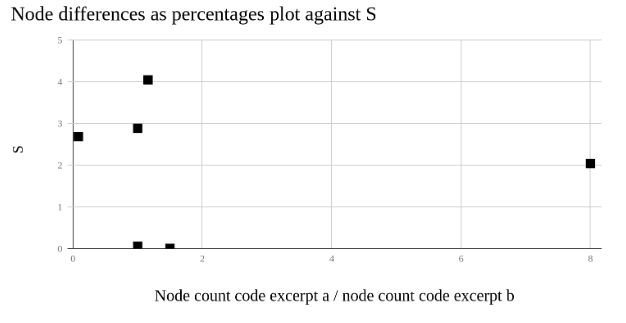
\includegraphics[width=0.50\textwidth]{nodecount}
\end{figure}

				\begin{figure}[h]
\caption{Key count similarity graph}
\centering
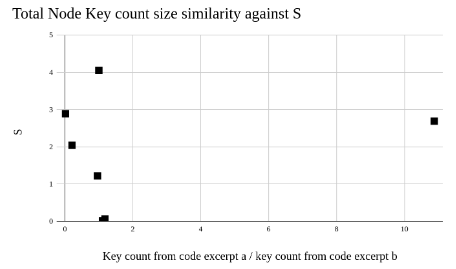
\includegraphics[width=0.50\textwidth]{keycount}
\end{figure}

Although generally a greater similarity in length of both keys and nodes in more similar code comparison can be observed, this perhaps what we would expect. The strength of this correlation has not been judged to be worrying and it is by no means the primary weight in comparison, in fact test 13 was engineered to have both identical node count and identical key count, this actually has the highest rate of dissimilarity in both Figure 6 \& 7. Hopefully dismissing the aforementioned concerns.

\subsection{Diff Values - Test Suite 2}
\textbf{Table 3} - Each letter in the diff value represents the difference type (D)eletion, (N)new, (E)dit, (A)rray Change. the number column headings refer to the JavaScript comparisons listed above. The cells are populated with the resulting $S$

\setlength{\tabcolsep}{1pt}
\renewcommand{\arraystretch}{1.5}

\begin{center}
 \begin{tabular}{||c c c c c c c c ||} 
 \hline
 Diff Values & 10 & 11 & 12 & 13 & 14 & 15 & 16 \\ [-0.2ex] 
 \hline\hline
 D=10,N=10,A=5, E=2.5 & 2.3 & 1.54 & 2.56 & 5.32 & <0.01 & 0.07 & 1.57 \\ 
 \hline
 D=10,N=10,E=2.5,A=1  & 2.18 & 1.54 & 2.56 & 5.32 & <0.01 & 0.01 & 1.57  \\
 \hline
 D=5,N=5,E=1,A=1  & 1.95 & 1.35 & 2.39 & 5.02 & <0.01 & 0.01 & 1.52  \\
 \hline
  D=10,N=10,E=1,A=0.2  & 1.93 & 1.35 & 2.39 & 5.02 & <0.01 & <0.01 & 1.52  \\
  \hline
    D=3,N=3,E=1,A=0.5  & 1.58 & 1.1 & 1.93 & 4.01 & <0.01 & 0.01 & 1.22 \\
  \hline
\end{tabular}
\end{center}

Enough has been said about diff values, the results are arranged in the order of heuristic effectiveness and the final row was chosen. In the case of test 16 which should ideally yield as $S$ of 0 this will be discussed as a limitation.

\clearpage

\section{Evaluation}
\subsection{JeSSE MOSS Differences}
To not unfairly malign either comparison system first their differences must be established so they can be accounted for in comparison.  MOSS does not identify plagiarism this is impossible, even a 100\% score on MOSS does not mean plagiarism has taken place, it is simply an indication. As MOSS was aimed to identify plagiarism even after students obfuscate code it functions differently than JeSSE which aims to identify similarities. Volunteer engineers, unlike assessed students,  have no incentive to hide if they have copied code.

Another feature of plagiarism is that often code is directly copied meaning lines may be identical other than some trivial changes to attempt to disguise this, volunteer engineers are not anticipated to copy, therefore JeSSE has been engineered to be more liberal in its similarity identification than it’s plagiarism detecting counterparts. MOSS JavaScript JeSSE differences: 

\begin{itemize}
  \setlength\itemsep{-0.5em}
  \item MOSS checks comments whereas JeSSE ignores them completely 
  \item MOSS cannot find any similarity between let/const declarations
  \item MOSS works on a percentage basis, with 100\% being the most similar. However this does not mean identical code will yield a 100\% rating. The longer the matching n-gram found the higher this value is.
  \item JeSSE's Transformed Similarity $TS$ works on a basis where 100 is the most similar and has no lower boundary, anything below 0 is displayed as 0. Although it should be remembered this is not percentage based, simply for similarity in comparison and clarity to engineers. 
\end{itemize}

To homogenise the comparison somewhat, MOSS's unilateral similarity values have been averaged as occurs in JeSSE. Additionally JeSSE's $TS$ value will be used rather than $S$ this more closely resembles MOSS's similarity value. These comparisons are not to discredit one system and bolster the reputation of the other, they are simply to see how they compare in the circumstances relevant to JeSSE. As mentioned previously, test suite 1 (Listing 6 - 21) was designed for the comparison of JeSSE and MOSS.

\setlength{\tabcolsep}{4pt}
\renewcommand{\arraystretch}{1.5}

\begin{center}
 \begin{tabular}{||c c c c c c c c c c||} 
 \hline
  & 1 & 2 & 3 & 4 & 5 & 6 & 7 & 8 & 9 \\ [-0.2ex] 
 \hline\hline
 JeSSE & 100 & 67.5 & 100 & 72.3 & 100 & 0 & 100 & 67 & 100 \\ 
 \hline
 MOSS  & 75\% & 0\% & 91\% & 0\% & 94\% & 0\% & 0\%  & 0\% & 0\%\\
 \hline
\end{tabular}
\end{center}

In test 1 some idea of how the systems compare, MOSS yields a 75\% score and JeSSE a 100 score for identical code. If this code is expanded to its state in 3 we see that the MOSS value increases to 91\% whereas JeSSE remains at its maximum similarity value of 100. If now symmetry is broken  of the compare functions where the systems differ becomes evident, in test 4 semantically equivalent code is compared MOSS finds “no matches” which will be referred to as 0\% after this point, whereas JeSSE's AST based comparison although somewhat thrown off by a few additional nodes yields at 72.3 similarity. The "program smell" these code excerpts are extremely similar and JeSSE has successfully managed to identify this similarity more successfully than MOSS. 

In test 5 a somewhat realistic hyper-simplified version of what may be seen in integration is present, both systems perform excellency in identifying the similarity here. All of the aforementioned comparisons have been working to identify short similar code, what if both systems are fed longer and much more dissimilar code? In test 6  code that shares minorly similarities but is generally very different is fed to the systems, both of these functions are taken from real integrations. Both systems identify this successfully with each provided its lowest score possible. 7 is an example with real applicability, the body of an integration (barry.js) is compared with itself but with its order scrambled. Even though the code in both functions is identical other than location, MOSS yields 0\% at all whereas JeSSE identifies a 100\% match. In test 6 the benefits of function inlining are visible, MOSS yields that there is no match between the two pieces of code, whereas JeSSE identifies that there is a strong similarity at 66. The 34 difference arises from the additional return statement (see Listing 35) along with the expression \texttt{b(value)}.

\begin{lstlisting}[caption= Test 6 with function inlined]
	let value = 50;
return b(value);
if (x > y) {
    return value * 2;
} else {
    return 0;
}

\end{lstlisting}

Test 8 demonstrates how the more liberal similarity comparison of JeSSE functions compared to MOSS. We see MOSS does not identify any similarities whereas JeSSE believes these are identical, this is seemingly a matter software similarity intent. 

\subsection{Comparison Efficiency}

Due to the nature of JeSSE not making use of hashing for comparison instead opting for the exclusive match algorithm which processes in quadratic time, concerns were raised about how the algorithm would scale in terms of runtime. Figure 8 is a graph documenting the homogenous growth of the size of each function. To balance the processing time between different types of code comparison was made using repeated lines listed below. As the hierarchy is built for every node in both trees order is irrelevant to processing time. Time is measured internally and measurements were taken 5 times for each and the mean was used.

\begin{figure}[h]
\caption{JeSSE Runtime with symmetrically increasing code size, i.e. code excerpt a and b are the length specified}
\centering
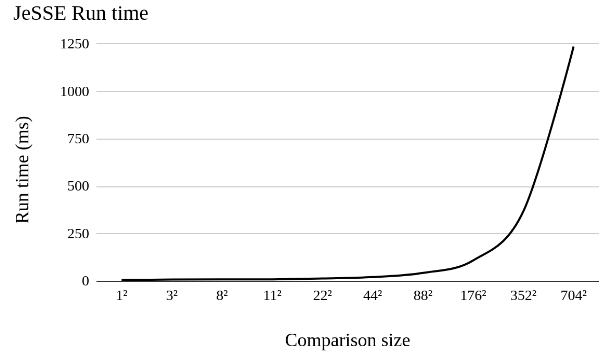
\includegraphics[width=0.5\textwidth]{jesseefficiency}
\end{figure}

Despite this rate of increase appearing minorly worrying it should be noted that these numbers are not for the entire module, but the body of each compare function. Currently, the longest integration (entire module) is under 300 lines, as there are 3 interface functions it is imagined be highly unlikely that the majority of these functions would reach even 200 lines. However what should be noted is that as these comparisons take place between each interface function of the new module and all other integrations, meaning 3 comparisons (albeit one trivial, \texttt{disconnect} is often essentially empty). If integration count was to reach over 100 this may start taking a toll. However, as code analysis is predicted to only be run on occasion this was considered completely reasonable.

\subsection{Limitations}
 In test 16 reveals a limitation of JeSSE, it cannot equate deprecated ECMAScript with new ECMAScript. As although these two code excerpts are identical in purpose they produce nodes with different keys, which is what the entirety of JeSSE functions off, although this provides great flexibility of the system in many circumstances it also limits it in this regard. Another example of where JeSSE performs poorly is in dissimilar code that performs a similar purpose, as JeSSE does not execute code this is a potential avenue for expansion.
 
 Combinatorial tuning of hyperparameters is highly desirable, a convincing argument can be made that the current tuning strategy is flimsy and biased although the use of a heuristic has helped with this. Tuning one parameter at a time leads to the issue that the parameters are agnostic to the other parameters, even if missing modifier calculation values are removed entirely all this will achieve is optimising diff values under that circumstance, there is no guarantee that the tuning performed under this circumstance holds up very effectively. However, the heuristic provided has ultimately been significantly improved so it is regarded as having some improvement even if perhaps the hyperparameters are far from their optimal values.  Ultimately this down to the oracle problem brought about as a result of the problem of similarity.
 
\subsection{TIDE}
TIDE offers a domain-specific-feature rich lightweight web IDE. The system supports, as specified, all variants of JavaScript execution and has never been found to take more than 3000 ms to execute when the latency is within reasonable bounds. TIDE is regarded to be a significant improvement over the previous developer playground and with the now built-in code similarity features, it is believed it will have a non-trivial reduction on the difficulty of developing an integration.
 
 \clearpage
\section{Future Work}

\subsection{JeSSE}
 JeSSE effectively identifies similar functions much like modern plagiarism tools, human input is still required to see if such similarities are sensible. The next steps for JeSSE could involve finding very similar subtrees seen in many integrations and then providing both volunteer and \textit{Tomorrow} engineers with the ability to view “suggested templates”. Volunteer engineers could verbatim insert these templates into their code and edit them however they see fit.  \textit{Tomorrow} Engineers could then perhaps consider adding them to some form of “templates library” allowing future engineers to browse these before implementing anything themselves, essentially reducing the boilerplate code required for the volunteer engineers to write. 

In the not so distant future perhaps many more engineers may see a template library built into their IDE hooked up to some monolithic database offering them suggestions on how other engineers have solved a similar problem. Either from their companies codebase or a global repository.

Finally, an important question has been raised as of yet unaddressed, what is software similarity? Future research may work to formalise a definition of software similarity solving the problem of similarity, although this will certainly not be easy to accomplish. 

\subsection{TIDE}
There are many areas for improvement, one of which is although the code is ran using the up to date resources, it is not at any point executed in their react native environment. Although no issues are foreseen here it is unlikely that no issues will arise from this in the long run. A solution to this would be to implement a new capability that extracts their code, injects it into the React Native codebase, builds and then runs the entire application on either a device the volunteer engineer has connected or an in-browser emulator. 

Another issue is it anticipated many developers will favour their standard desktop IDEs as they are more accustomed to them and they provide more features even at the expense of domain-specific features. Ideally in the future for such developers who are not simply playing around with the idea of building an integration but developing a substantial module the development environment would be able to link up with the IDE. The idea of a web IDE has certainly not encountered into as many hurdles as anticipated, but as many engineers are accustomed to their IDE's it may more difficult to get engineers to migrate for non-domain-specific purposes. 

A final feature idea that would remove the only remaining toil would be to automate a pull request with the open-source GitHub repository.

\clearpage

\section{Conclusion}
TIDE is believed to be a highly functional IDE offering a number of domain-specific capabilities that are hoped to encourage more volunteer engineers to get and remain involved with climate activism via the use of their technical skills. JeSSE has been shown to perform remarkably well when compared to its plagiarism detecting cousins, it is hoped that it will see widespread use within this small community of volunteer engineers. If so its usefulness will only grow as that community continues to expand. 

\bibliography{references}


\end{document}
